\documentclass[border=2pt]{standalone}
\usepackage{tikz}
\usepackage{amsmath}
\begin{document}
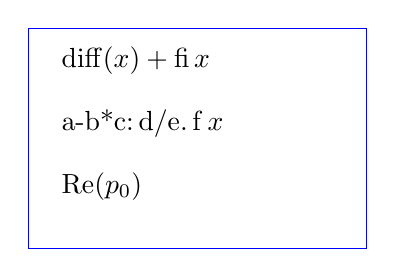
\begin{tikzpicture}
  \draw[blue] (-.3,.5) rectangle (4,-2.3);
  \node[anchor=base west] at (0,0) {$\operatorname{diff}(x)+\operatorname{fi}x$};
  \node[anchor=base west] at (0,-.8) {$\operatorname{a-b*c:d/e.f}x$};
  \node[anchor=base west] at (0,-1.6) {$\operatorname{Re}(p_0)$};
\end{tikzpicture}
\end{document}
